\chapter{Application: font glyph generation}\label{chap:training} To demonstrate our end-to-end SVG generation method, we train the model architecture described in Chapter~\ref{chap:architecture} on a dataset of font glyphs.

\section{Dataset}\label{sec:font-data}
Our dataset of font faces is downloaded from a GitHub repository containing all fonts available on Google Fonts (\url{https://github.com/google/fonts}).
The dataset contains 2552 font faces total from 877 font families.
Font faces exhibit much stylistic variation: a breakdown of font types for the 877 font families can be found in Table~\ref{tbl:fonttypes}, and examples of font glyphs from each type can be found in Figure~\ref{fig:fonttypes}.

\begin{table}[h]
\centering
\caption[A breakdown of font types in the Google Fonts dataset]
    {The 2552 font faces in the Google Fonts dataset are from 877 total font families.
    Each font family can be classified as one of the following categories, with the ``display'' category encompassing bold fonts of a wide variety of styles that can be used as title text.
    Here, we report the counts of font families in the dataset belonging to each type.\label{tbl:fonttypes}}
\begin{tabular}{c c c c c}
\toprule
    Serif & Sans serif & Display & Handwriting & Monospace \\ \midrule
    180 & 249 & 296 & 135 & 17
\end{tabular}
\end{table}

All font faces are downloaded as TrueType (TTF) files then converted to SVG format using the FontForge command-line tool\footnote{\url{https://fontforge.github.io}}.

Input statistics highlighting the number and type of SVG commands within drawings for the glyph \textbf{b} across all font faces are shown in Figure~\ref{fig:stats-b}.
The remaining glyph statistics can be found in Appendix~\ref{app:data}.

\begin{figure}[h]
    \caption[Dataset statistics for the glyph \textbf{b}]
    {Dataset statistics for the glyph \textbf{b} across all 2552 font faces in the Google Fonts dataset.\label{fig:stats-b}}
\centering
    \subcaptionbox{A histogram depicting the number of feature vectors used to encode glyphs of the character \textbf{b} across our font faces.
    The glyph \textbf{b} has, on average, 91 feature vectors in its representation.
    Glyphs with more than 250 feature vectors were left out of our dataset when training.
    }
{\begin{tikzpicture}
\begin{axis}[
 	xlabel={feature vector count},
    ylabel={number of \textbf{b} glyphs},
	width=0.45\textwidth,
    ybar,
    ymin=0
]
\addplot [
	fill=color1,
	fill opacity=0.4,
    hist={
        bins=7,
        data min=0.5,
        data max=300
    }   
] table [y index=0] {data/b_points_stats.csv};
\end{axis}
\end{tikzpicture}
}\quad
    \subcaptionbox{A breakdown of the occurrences of line and quadratic B\'ezier drawing commands per glyph.
    Note that TTFs support only these two types of drawing commands, although  SVGs in general can contain any of the commands listed in Table~\ref{tbl:svg-commands}.
    }
{\begin{tikzpicture}
\begin{axis}[
 	xlabel={command type count},
    ylabel={number of \textbf{b} glyphs},
	width=0.45\textwidth,
    ybar,
    ymin=0
]
\addplot [
	fill=color2,
	fill opacity=0.4,
    hist={
        bins=7,
        data min=0.5,
        data max=100
    }   
] table [y index=0] {data/b_line_count.csv};
\addplot [
	fill=color3,
	fill opacity=0.4,
    hist={
        bins=7,
        data min=0.5,
        data max=100
    }   
] table [y index=0] {data/b_quad_count.csv};
\addlegendentry{\code{line}}
\addlegendentry{\code{quad}}
\end{axis}
\end{tikzpicture}
}
\end{figure}

\section{Training}\label{sec:training}
We train a separate instance of the model for each of the glyphs \textbf{b}, \textbf{f}, \textbf{g}, \textbf{o}, and \textbf{x}, chosen because they cover a variety of shapes and curves.
Each input SVG is transformed to a list of feature vectors using the method described in Chapter~\ref{chap:features}.
We use encoding B to translate SVG commands to feature fectors, details of which are described in Chapter~\ref{chap:feature-variation}.
The datasets are then randomly partitioned into training, test, and validation sets; glyphs from the overall dataset of 2552 font faces are pruned if they consist of more than 250 feature vectors.
Every glyph except \textbf{x} has a training set of 1920 SVGs, while \textbf{x} has a training set of 1960.
All glyphs have test and validation sets of 240 SVGs each.
Training is done with a batch size of 40, a learning rate of 0.001, and a KL weight in the loss function that starts at 0.01 and increases asymptotically over time.
The size of the latent space vector $z$ is set to 128, and we use recurrent dropout to reduce overfitting.
Loss graphs and details about trained models can be found in Appendix~\ref{app:train}.

\section{Results}
Here, we report quantitative results as well as a qualitative evaluation of model performance.
In Figure~\ref{fig:font_gen}, we highlight ground truth inputs and their conditionally decoded outputs for each of the letter glyph models.
\begin{figure}[h]
    \centering
	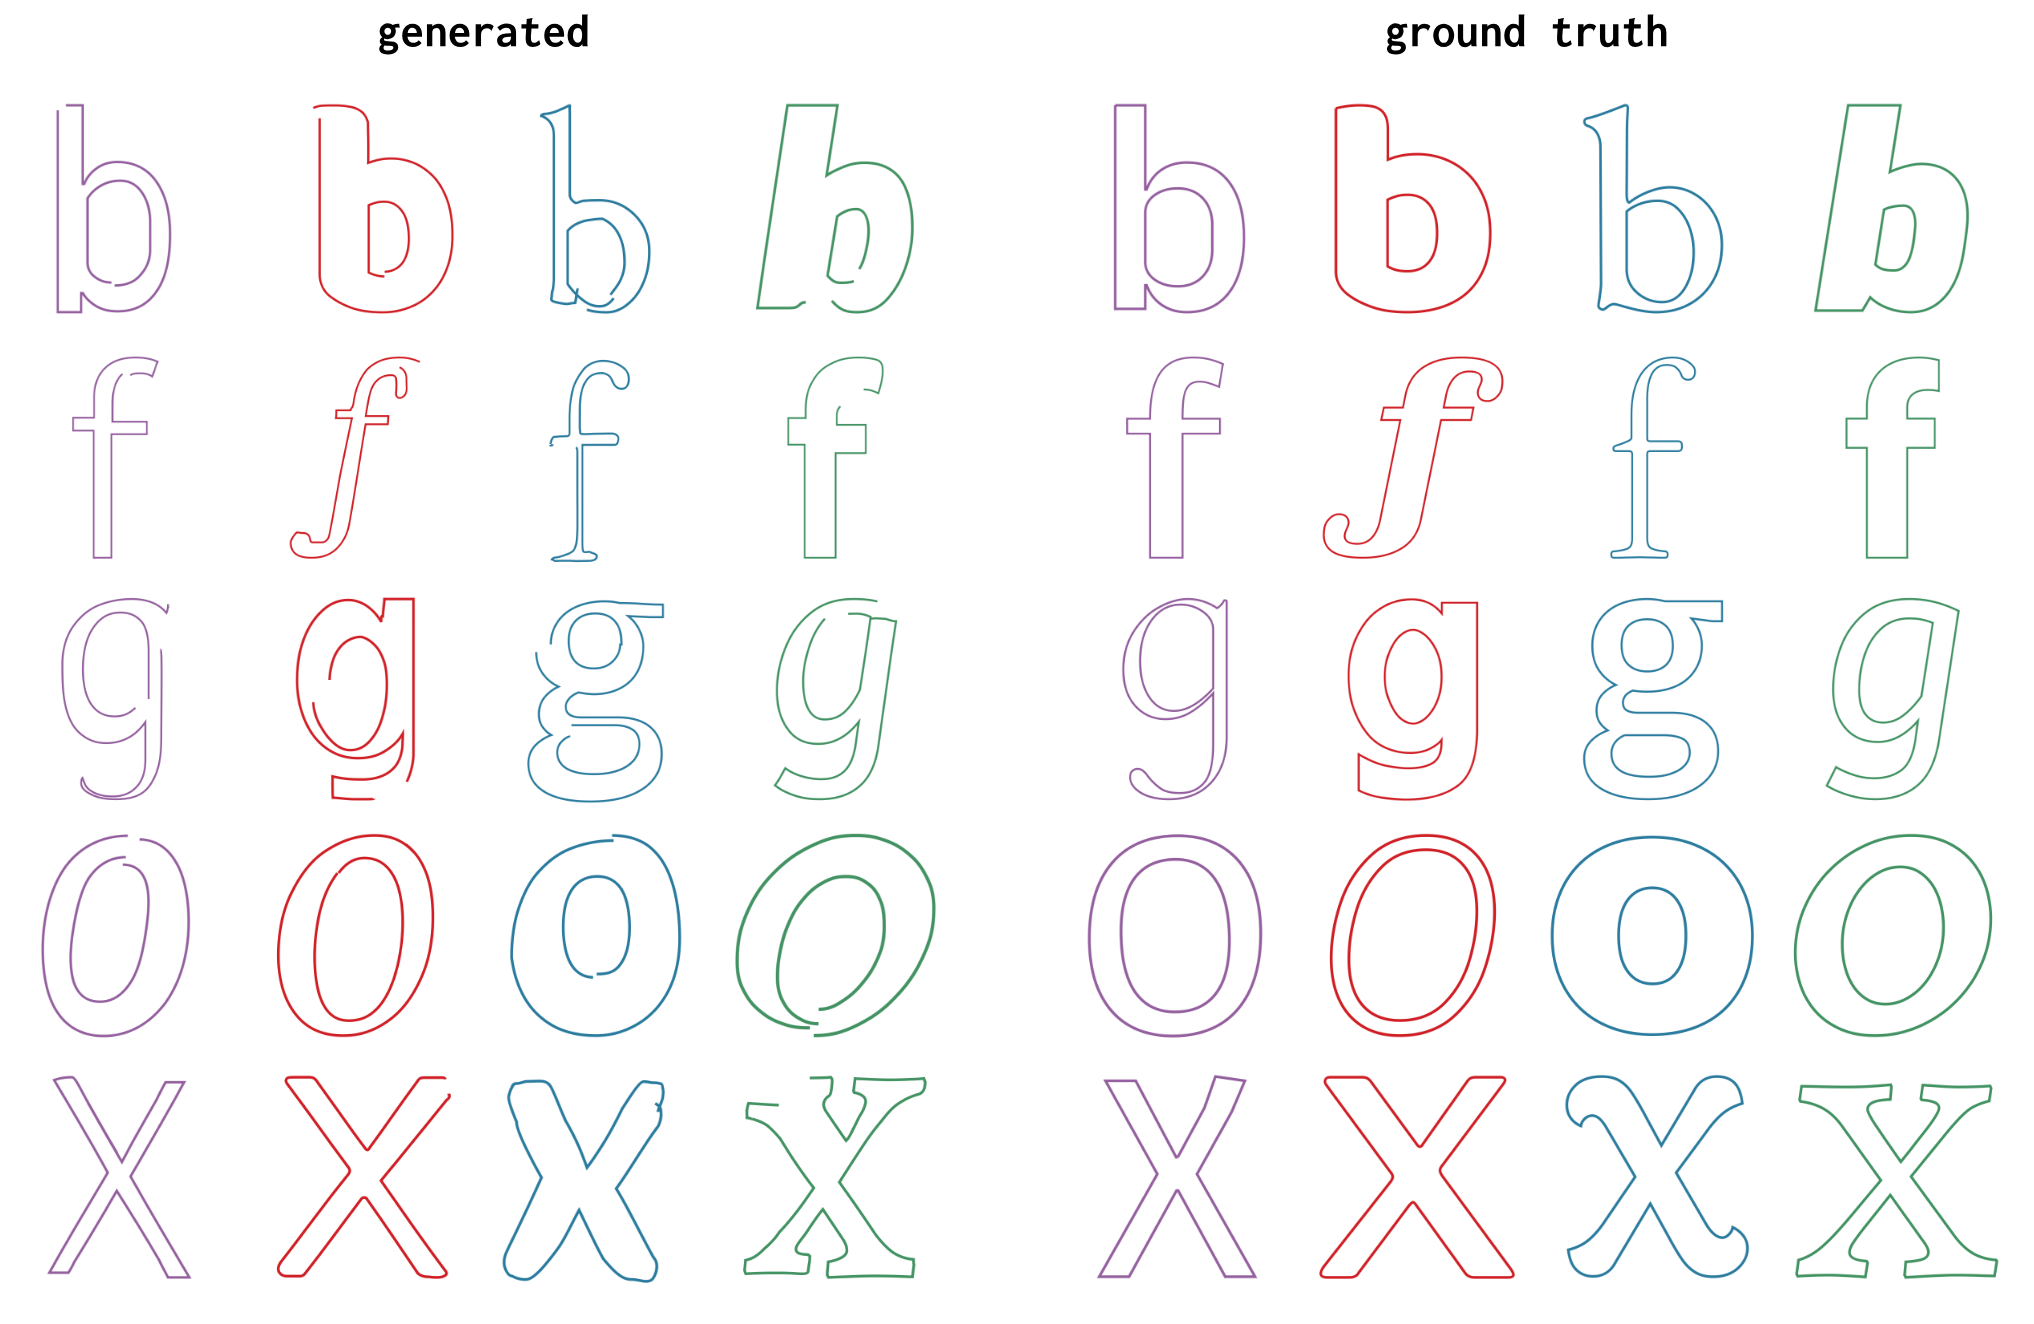
\includegraphics[width=\textwidth]{figures/font_gen}
    \caption[Visual results of training single-class model on letter glyph datasets]
    {Selected glyphs conditionally generated by the trained single-class letter glyph model.
    Ground truth inputs on the left are fed into the encoder and decoded into the generated outputs on the right.\label{fig:font_gen}}
\end{figure}

\subsection{Quantitative results}\label{sec:quant-eval}
\begin{table}[h]
\centering
\caption[Quantitative results for models trained on letter glyphs]
    {Modified Hausdorff distance for models trained on each glyph on a test set of $N$ images.
    We also provide two baselines: one comparison between input images and random noise with the same dimensions (to provide a reasonable upper bound), and one comparison between randomly sampled pairs of the same glyph class.
    \label{tbl:model-results}}
\begin{tabular}{c c c c c}
\toprule
    Glyph class & Mean & Std.\ dev. & Kurtosis & $N$ pairs \\ \midrule
    \multicolumn{5}{c}{Conditionally generated vs.\ ground truth} \\ \midrule
    \textbf{b} & 19.5341 & 8.3484 & 1.9515 & 240 \\
    \textbf{f} & 15.7533 & 9.2132 & 4.7359 & 240 \\
    \textbf{g} & 19.7714 & 9.6469 & 6.8383 & 240 \\
    \textbf{o} & 27.8857 & 11.9887 & 5.8081 & 240 \\
    \textbf{x} & 28.8542 & 14.2474 & 1.9820 & 238 \\ \midrule
    \multicolumn{5}{c}{Random noise vs.\ ground truth} \\ \midrule
    \textbf{b} & 180.9758 & 18.7591 & 27.0412 & 240 \\
    \textbf{f} & 188.4756 & 40.3329 & 2.7637 & 240 \\
    \textbf{g} & 185.9078 & 31.1026 & 3.7460 & 240 \\
    \textbf{o} & 204.1991 & 21.1567 & 2.91859 & 240 \\
    \textbf{x} & 188.7353 & 16.9588 & 0.1258 & 240 \\ \midrule
    \multicolumn{5}{c}{Random ground truth pairs} \\ \midrule
    \textbf{b} & 23.2421 & 12.8087 & 2.8928 & 120 \\
    \textbf{f} & 26.8287 & 13.0423 & 2.7861 & 120 \\
    \textbf{g} & 24.6996 & 11.2764 & 6.9264 & 120 \\
    \textbf{o} & 25.1075 & 13.5501 & 3.9498 & 120 \\
    \textbf{x} & 21.8579 & 9.1399 & 1.0702 & 120 \\
\end{tabular}
\end{table}

To quantify model performance, we compute an image similarity metric between each ground truth image and a corresponding image conditionally generated by the model with $\tau = 0.3$, where temperature $\tau$ specifies randomness when sampling from the decoder as defined in~\cite{ha2017neural}.
Images are first converted to point clouds containing every pixel in the raster image with nonzero value.
The resulting sets of points are translated to be mean-centered for each image, and the modified Hausdorff distance in the range $[0, \infty\}$ is calculated from the point set of each generated image to the point set of its corresponding ground truth image~\cite{dubuisson1994modified}.
While we also considered using metrics such as pixel loss and feature extraction, we chose the Hausdorff distance for its simplicity as a measure of mutual polygonal proximity.
Evaluation is run on a set of $N$ test images for each glyph, and quantitative results can be found in Table~\ref{tbl:model-results}.
We also provide baselines for the Hausdorff metric: one comparison between input images and random noise with the same dimensions, and one comparison between randomly sampled pairs of the same glyph class.

\subsection{Qualitative results}
We demonstrate the model's learned ability with a few illustrative examples.

In Figure~\ref{fig:interp}, we interpolate between latent vectors for input \textbf{b} and \textbf{f} glyphs of different styles.
If interpolated latent vectors tend to produce coherent outputs, it indicates that the KL regularization term in the loss function is sufficiently forcing the latent space to be used efficiently.
\begin{figure}[h]
    \centering
	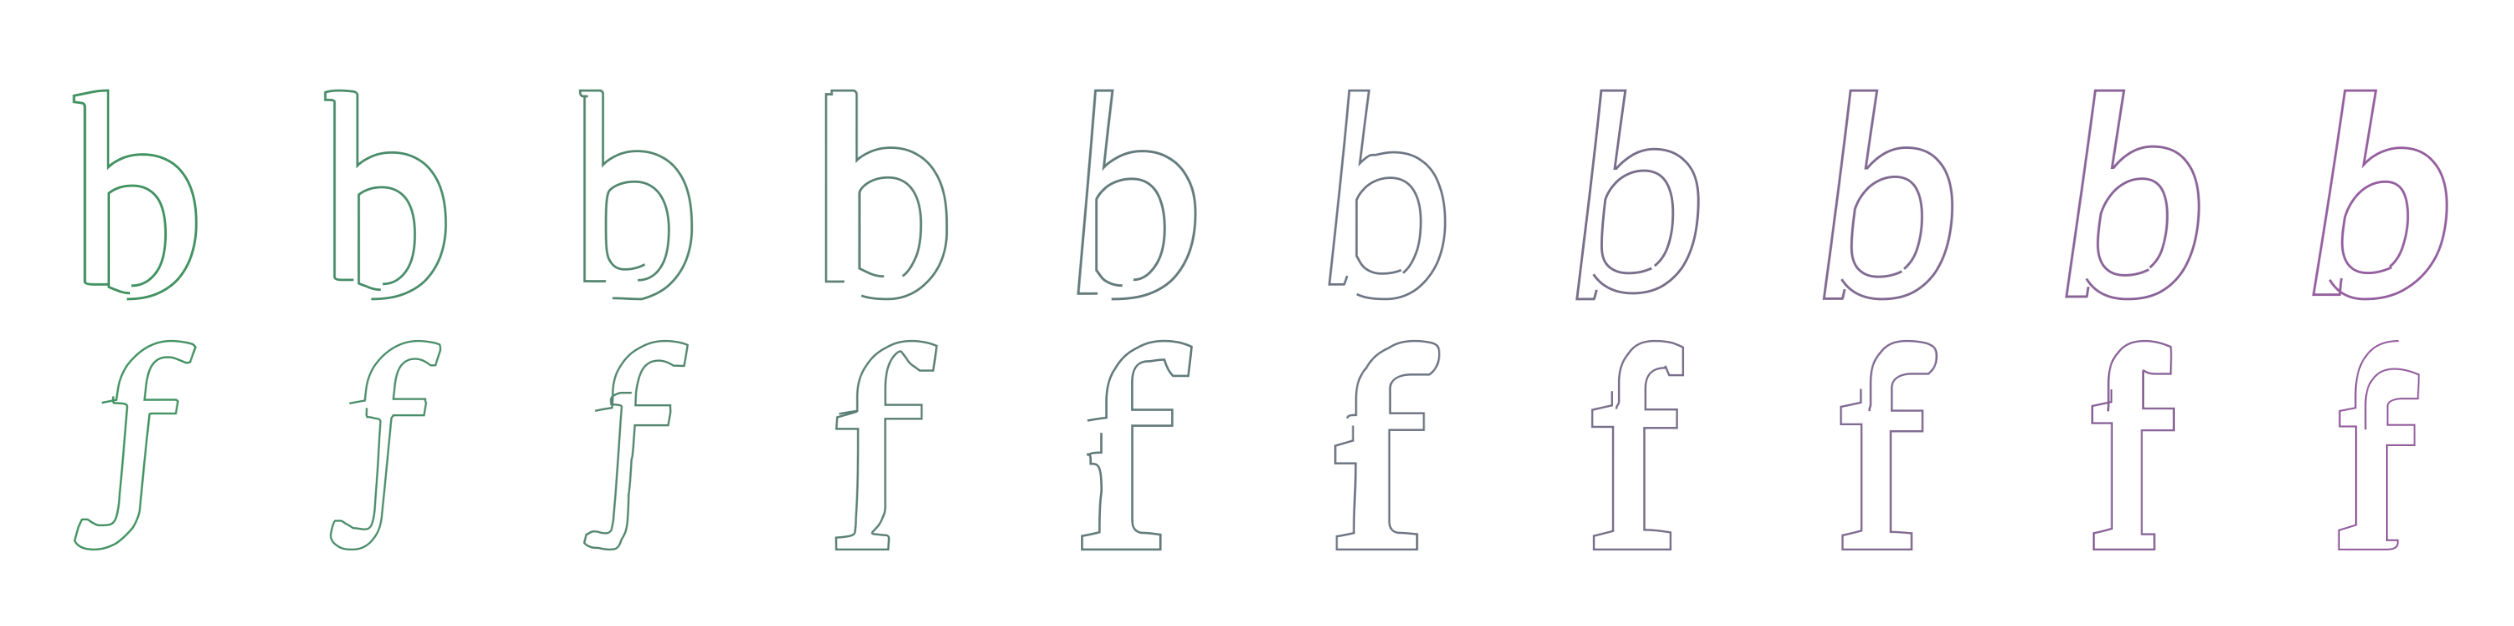
\includegraphics[width=\textwidth]{figures/interp}
    \caption[Latent space interpolation for the single-class model]
    {The latent space abstractly encodes style and must learn to identify different types of glyphs.
    The input glyphs are on the far sides of the figure, and we spherically interpolate between their latent vectors, decoding with $\tau=0.1$.\label{fig:interp}}
\end{figure}

In Figure~\ref{fig:temp}, we demonstrate how temperature $\tau$ affects the decoding process as a randomness scaling factor in sampling from the decoder output GMMs.
Intuitively, a lower temperature indicates that the decoder samples outputs that it believes are more likely.
\begin{figure}[h]
    \centering
	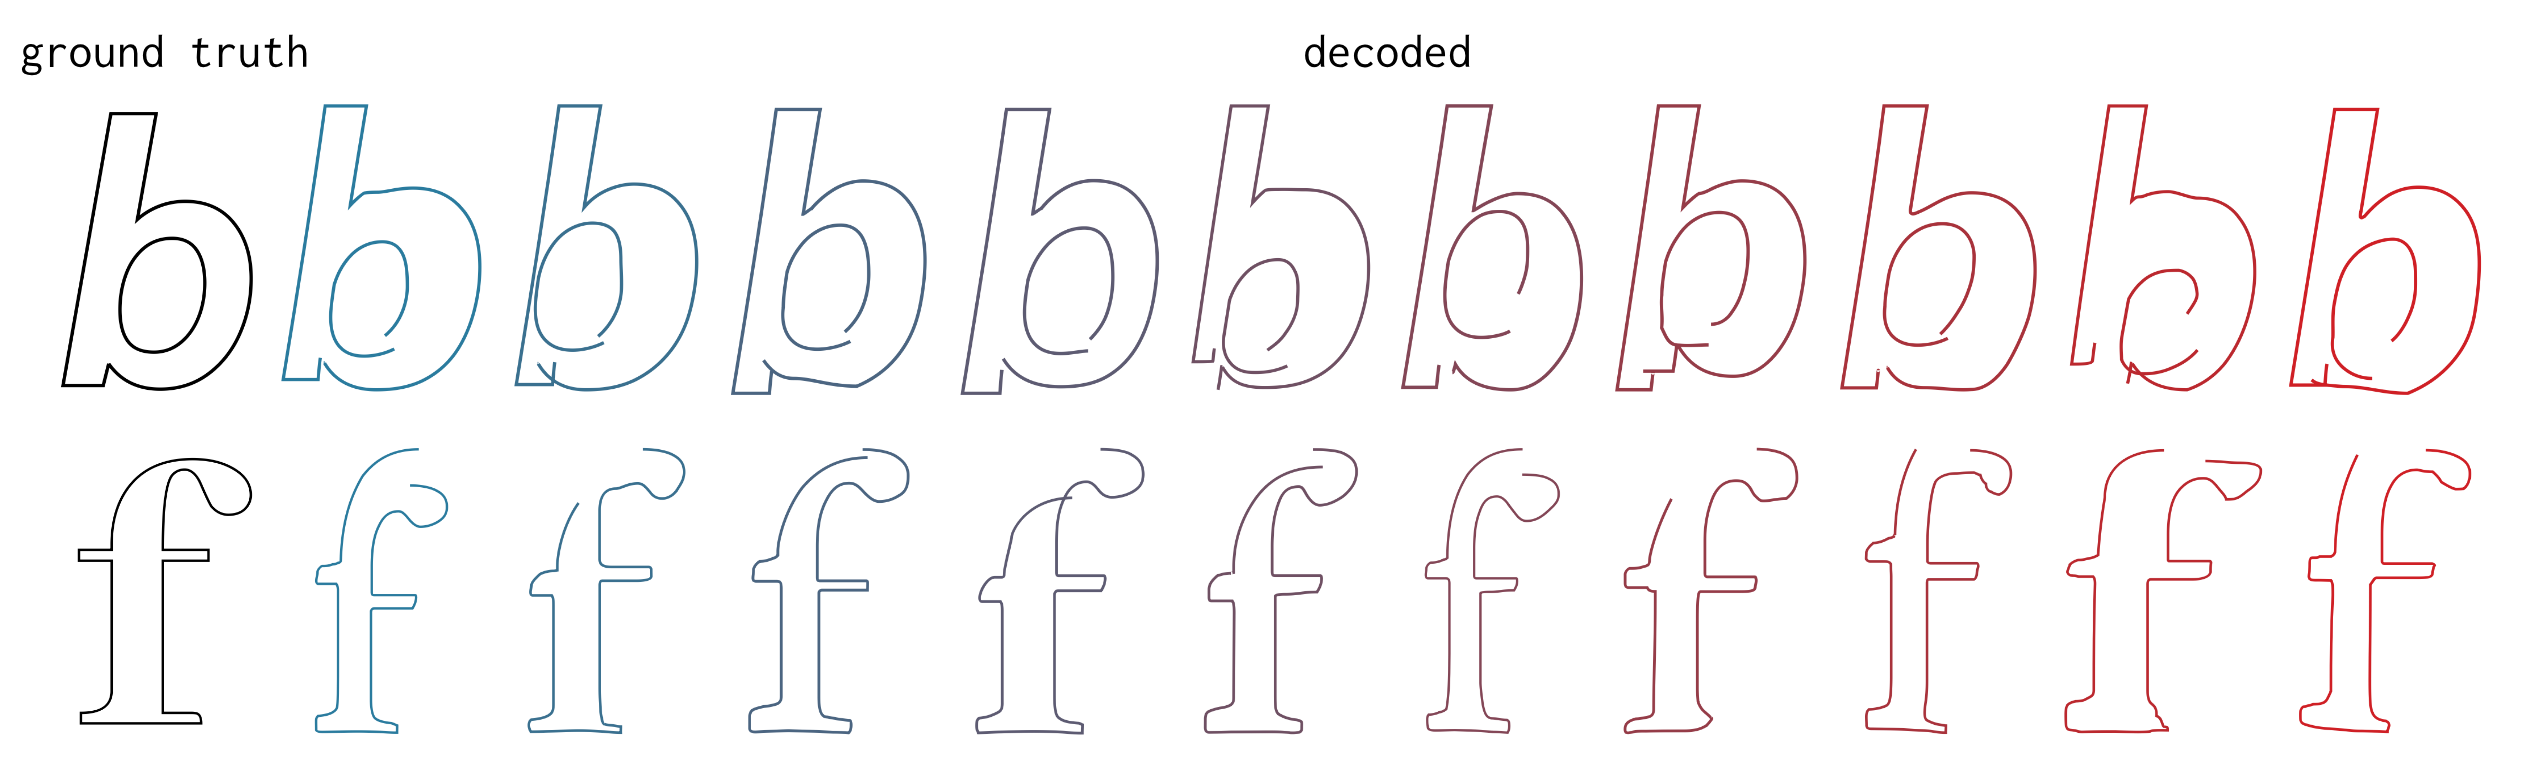
\includegraphics[width=\textwidth]{figures/temp_grid}
    \caption[The temperature grid for a conditionally generated glyph]
    {To demonstrate how temperature affects decoding, we decode the same latent vector at different temperature settings.
    At the far left, $\tau=0.1$, and at the far right, $\tau=1.0$, with $\tau$ increasing by 0.1 for every intermediate image.
    As temperature increases, model generates outputs less likely to match the input image.
    \label{fig:temp}}
\end{figure}

Figure~\ref{fig:fails} depicts common failure modes during conditional generation.
Because the model is drawing sequences of commands using pen displacement, it often struggles with closing the loop and returning to its original path start point.
Additionally, since some font face styles are exceptionally rare, the model fails to learn how to represent non-standard font styles.
\begin{figure}[h]
    \centering
	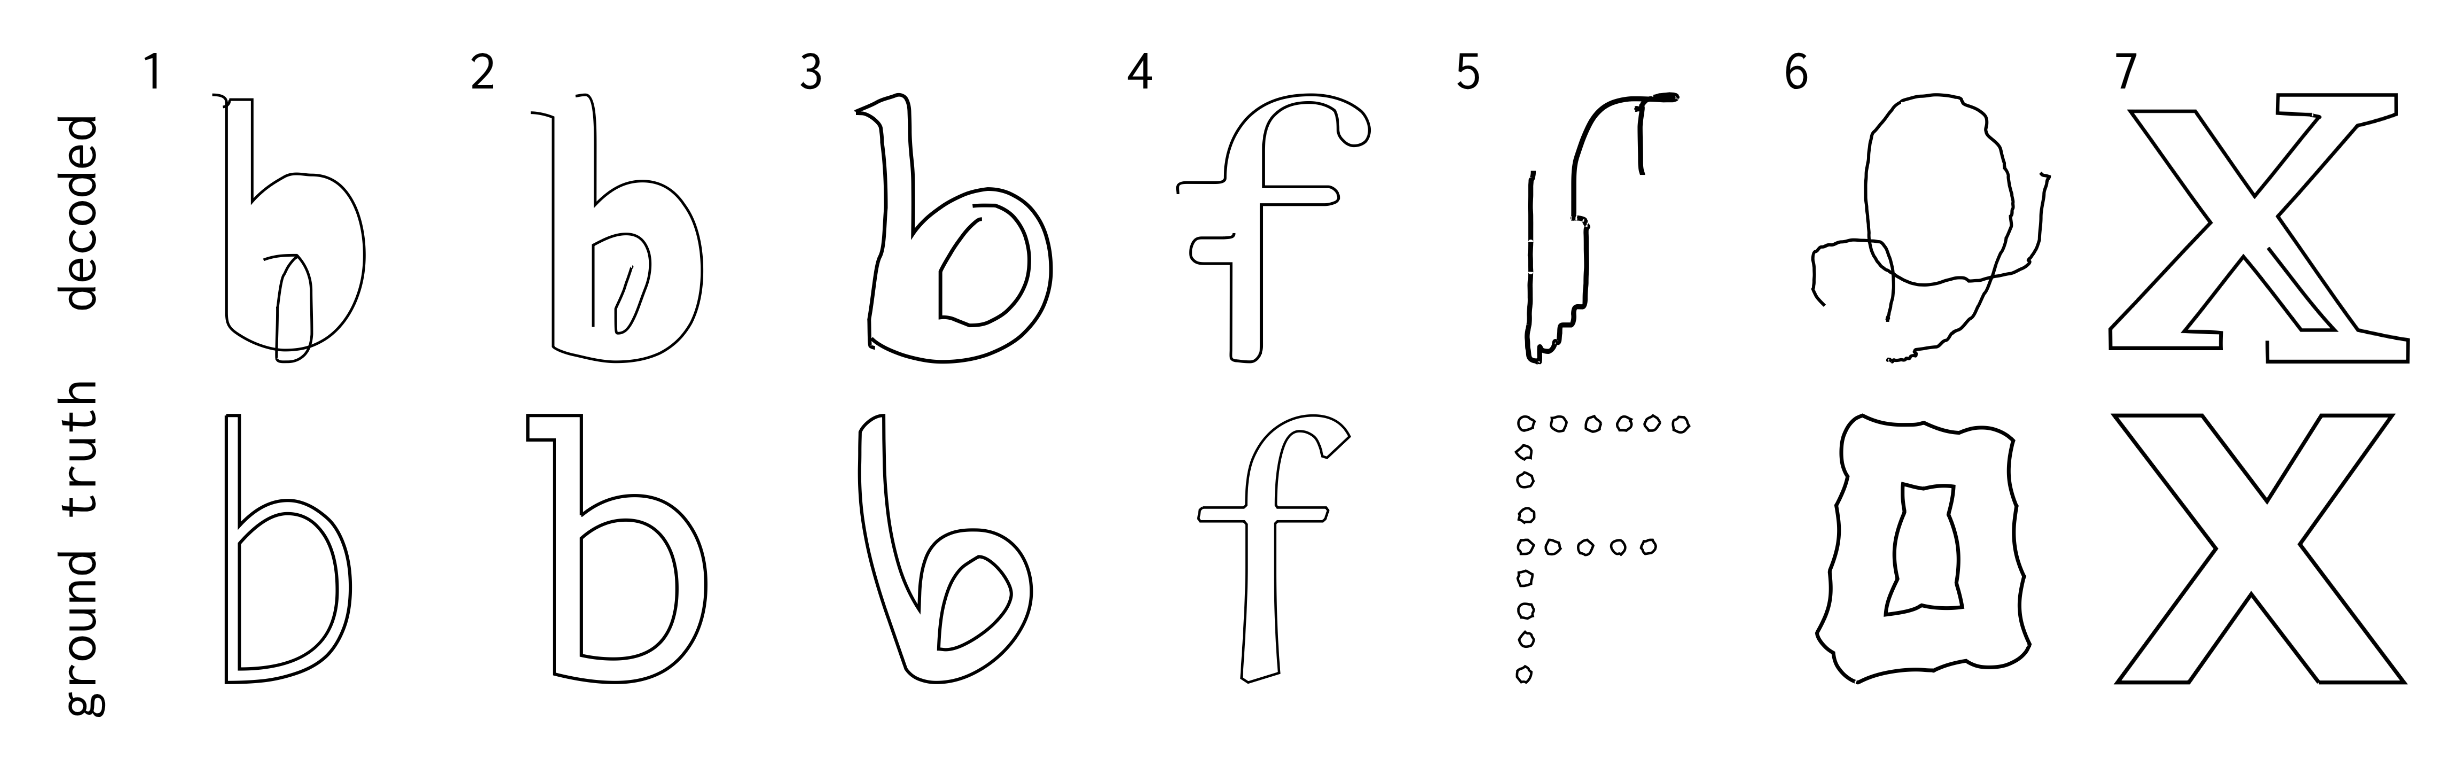
\includegraphics[width=\textwidth]{figures/fails}
    \caption[Common failure cases for conditional generation]
    {The model generally makes a set of common mistakes, as shown here.
    It struggles with positioning disconnected components (1), closing paths (2, 4), and understanding uncommon styles (3, 5, 6). It also sometimes confuses styles (7).\label{fig:fails}}
\end{figure}
\newpage

Finally, Figure~\ref{fig:uncond} demonstrates the creative ability of the model: generating unseen examples of a variety of styles.
Instead of encoding an input SVG and passing in the resulting latent vector into the decoder, we train the decoder separately to learn unconditional generation without a $z$ input, with the decoder RNN initial states instead set to 0.
\begin{figure}[h]
    \centering
	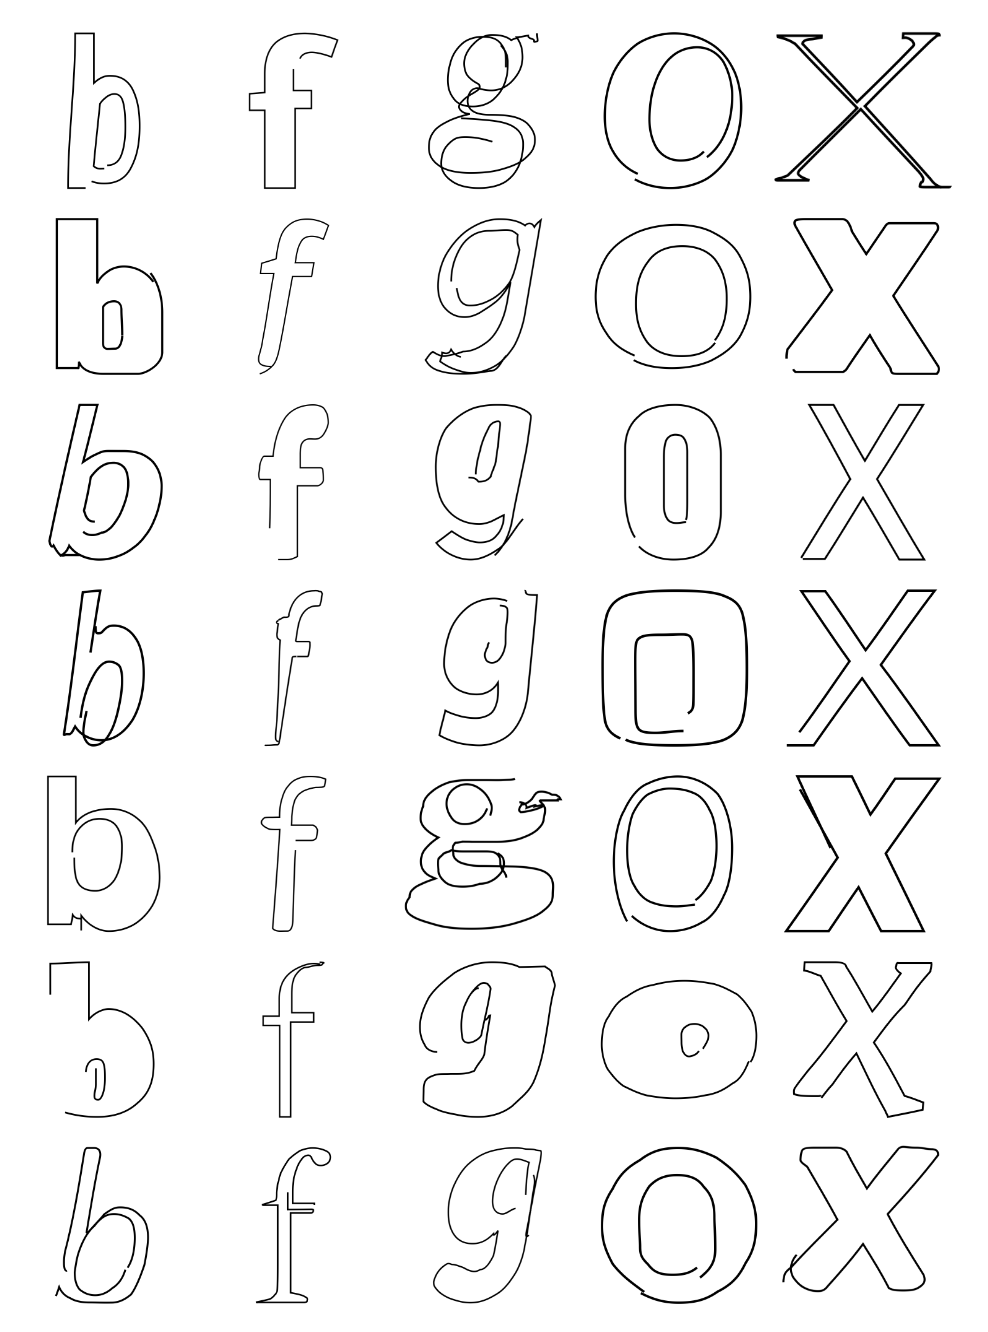
\includegraphics[width=\textwidth]{figures/uncond}
    \caption[Unconditional generation for the single-class model on letter glyphs]
    {We generate novel, unseen examples by training the decoder only without any latent variable input, feeding only the previously generated command into the decoder cells.
    The decoder is run with initial states set at 0, and sampling outputs is done at $\tau=0.01$.
    \label{fig:uncond}}
\end{figure}
